

\section{Sparse Input processing}

%% methods deal with sparse input, like nconv, gconv ...
The depth map is supposed to be dense. Therefore, how to accept sparse depth map as input in CNNs is one of the most important problem. Some trivial solutions like median filters are good enough, if the missing pixels are sparse enough, however, for the case of huge missing holes in the depth map, it produces just a paltry result. Thus a reasonable guess is required for missing areas. Generally, it can be solved as image inpainting problems,\cite{inpainting1},\cite{inpainting2}. 

%% Deep learning based approaches
Some deep learning based method for image inpainting also achieved quite good performance for the hole mending task. 
%% talk about gconv
Notably, in 2016, Oord et al. \cite{gated_activation} proposed a gated activation unit for a CNN model,
\[\textbf{y} = \tanh (W_{k,f} * \textbf{x}) \odot \sigma (W_{k,g} * \textbf{x})\]
to substitute the standard activation layer, where $ \sigma $ is the sigmoid function, which constricts the output value of second part between $ [0,1] $.  The function is inspired by Long Short-Term Memory (LSTM) \cite{lstm} and Rated Recurrent Unit (GRU).\cite{gru} It is originally used for learning complex interactions as LSTM gates does. In 2018, Yu et al. \cite{gconv} employed same function for free-form image inpainting, which can be used to learn mask automatically from image it self.

%% talk about nconv
Different to aforementioned approaches, Knutsson et al. in 2005 introduced normalized convolution \cite{nconv} dealing with missing sample case for convolution operation, which aims to reconstruct the missing pixels from the sparse output sensed by cameras, which particularly considered the confidence of each interpolated pixels, since it provides the trustworthiness of the predicted value. The higher the reliability of the value inference, the better the model shape reconstruction.

In 2018, Eldesokey et al. \cite{ncnn} applied normalized convolution in CNN as normalized convolution layer that takes both sparse depth map and a binary confidence map as input to perform scene depth completion.
In 2020, Eldesokey et al. \cite{pncnn} focus on modeling the uncertainty of depth data instead of assuming binary input confidence.

Guided method \cite{guided} requires addition information like RGB image or the certainty map of depth map, and fuse them together to predict the dense depth map.




\section{Normal Inference}

%% normal estimation method introduction
Usually, we based on point cloud, depth map or RGB/Grayscale image of the objects or scenes to inference the normals. 

Traditional methods evaluate normals based on neighbor information of point cloud or depth map.
In 2012, Holzer et al. \cite{Holzer.S} proposed method to calculate normal from covariance matrices. 
This method use integral image as input, which is able to run algorithm in a high frame speed. They smooth the depth data in order to handle the noise of depth image. The drawbacks are, as mentioned in the paper, the normals error go up when point depths change severely. In 2013, Fouhey et al. \cite{geometry_based_solution} proposed a method constructing a over-determined function systems to predict normals and solving it 
by algebra methods. Similarly, this approach gives a quick but coarse normal inference. 


%% CNN based methods
Recently, CNN based methods improve the performance of image processing to a brand new stage. In 2014, Eigen et al.\cite{Eigen} proposed a method predicting depth map directly from RGB image using CNN. In this case, no depth map is required. In 2016, Laina et al. \cite{img2depth} proposed a deeper network based on ResNet \cite{resnet} with a well designed upsamling part. 
%% guided scene completion
In 2018, Qi et al. proposed GeoNet\cite{GeoNet}, it integrates both algebra method and also CNN method to inference depthmap based on \cite{img2depth} \cite{geometry_based_solution}. 

%% upsampling 
It is worth to noticed that, the output of normal inference CNN model is not one or severl labels but an entire image or normal map with same size. 
%% talk about image upsampling, unet
Recently, Ronneberger et al proposed an architecture called UNet \cite{unet} for biomedical image segmentations. The architecture is shown in Figure \ref{fig:u-net}.The first half network is a usual classification convolutional network, the second half replace the pooling layers and traditional fc layers in the traditional CNNs to upsampling layers, thus in the end of the second half, the output is able to back to the input size. The proposed network can successfully assigned each pixel a class for segmentation tasks. Under this symmetric network, an input image is downsampled 3 times and upsampled 3 times. Output image has exactly the same size as input image. The downsampling and upsampling both have large number of feature channels, which guarantee the network propagates the information to higher resolution layers.


\begin{figure}[!h]
	\centering
	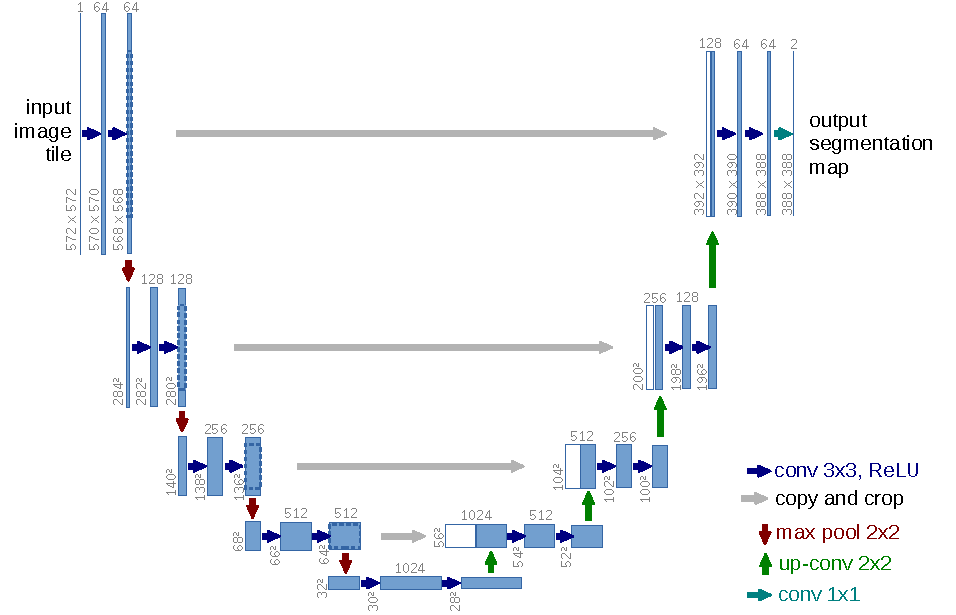
\includegraphics[width=\textwidth]{./ref/u-net-illustration-correct-scale2}
	\caption{U-net architecture (example for 32x32 pixels in the lowest resolution). Each blue box corresponds to a multi-channel feature map. The number of channels is denoted on top of the box. The x-y-size is provided at the lower left edge of the box. White boxes represent copied feature maps. The arrows denote the different operations.
	}
	\label{fig:u-net}
\end{figure}



%% unstructured point cloud 
In some case, the input is unstructured point cloud which can not be fed into a CNN entirely. Thus, a challenge task connect to the deep learning is the input format. Since different point clouds have different sizes. 
In 2018, Ben-Shabat et al. \cite{Ben-Shabat_2019_CVPR} presented Nesti-Net. It predicts the normal point by point with the help of neighbor points. It fixed the distance of considering neighbors to provide an unified input for CNN. In 2021, Zhou et al. \cite{zhou2021fast} presents a method considering overlapping of different patches (a group of neighboring points) as input to evaluate normals. 
 















